\documentclass[12pt,a4paper]{article}

% Cấu hình Tiếng Việt cho trình biên dịch mặc định (pdfLaTeX) trên Overleaf
\usepackage[T1,T5]{fontenc}
\usepackage[utf8]{inputenc}
\usepackage[vietnamese]{babel}

\usepackage{amsmath}
\usepackage{amsfonts}
\usepackage{amssymb}
\usepackage{graphicx}
\usepackage{hyperref}
\usepackage{booktabs}
\usepackage{geometry}
\usepackage{caption}
\usepackage{subcaption}
\usepackage{setspace}
\usepackage{float}

% Căn lề chuẩn
\geometry{
    a4paper,
    left=3cm,
    right=2cm,
    top=2.5cm,
    bottom=2.5cm
}

% Giãn dòng 1.25 hoặc 1.5 cho dễ đọc
\setstretch{1.25}

% Thiết lập hyperlink
\hypersetup{
    colorlinks=true,
    linkcolor=blue,
    filecolor=magenta,      
    urlcolor=cyan,
    pdftitle={Báo Cáo Tiến Độ Lần 01},
}

\title{\textbf{BÁO CÁO TIẾN ĐỘ LẦN 01}\\ 
\large \vspace{0.5cm} \textit{Dự án: Benchmarking TurboQuant and KV Cache Compression Methods on Vietnamese Large Language Models}}
\author{\textbf{Nhóm Thực Hiện:} Data Team \& Infrastructure Team}
\date{\textbf{Thời gian báo cáo:} Tháng 06 năm 2026}

\begin{document}

\maketitle
\newpage

\tableofcontents
\newpage

\section{Summary}

Dự án \textit{Benchmarking TurboQuant and KV Cache Compression Methods on Vietnamese Large Language Models} được thực hiện nhằm đánh giá và đo lường hiệu năng của các thuật toán nén Key-Value (KV) Cache, đặc biệt là TurboQuant, khi áp dụng vào các mô hình ngôn ngữ lớn (LLMs) dành riêng cho tiếng Việt. Ở giai đoạn hiện tại, trọng tâm của dự án là việc thiết lập hạ tầng thực nghiệm và xây dựng chuỗi xử lý dữ liệu (data pipeline) chuyên dụng. 

Tính đến thời điểm báo cáo, trạng thái chung của dự án được đánh giá là \textbf{Hoàn thành một phần}, ước lượng đạt khoảng \textbf{20\% tổng khối lượng tiến độ dự án}. Pipeline chuẩn bị dữ liệu (curation) đã được xây dựng thành công bao gồm cấu hình nền tảng Docker, các kịch bản tải dữ liệu tự động từ Hugging Face, và một backend linh hoạt tích hợp giữa framework NeMo Curator của NVIDIA và ngôn ngữ Python. Quan trọng hơn, nhóm đã phát triển các bộ lọc chuyên dụng cho đặc thù ngôn ngữ tiếng Việt. Kết quả ban đầu đã tạo ra được tập dữ liệu kiểm thử (test-set) cho ngữ cảnh dài (long-context). Bên cạnh đó, hạ tầng phần cứng cũng đã được thiết lập hoàn chỉnh, sẵn sàng cho các bước thực nghiệm chuyên sâu tiếp theo.

\begin{table}[H]
\centering
\begin{tabular}{@{}ll@{}}
\toprule
\textbf{Hạng mục công việc} & \textbf{Trạng thái hiện tại} \\ \midrule
Hạ tầng máy chủ (Host) & Hoàn thành \\
Cấu hình Docker Compose & Hoàn thành \\
Xác thực môi trường chạy Docker (Runtime) & Hoàn thành \\
Xây dựng tập Test-set JSON & Hoàn thành (12 samples) \\
Thu thập nguồn dữ liệu VTSNLP & Hoàn thành (5,000 raw records) \\
Thu thập nguồn dữ liệu VMLU \& V-Bench & Chưa hoàn thành (Gặp lỗi 401) \\ \bottomrule
\end{tabular}
\caption{Tóm tắt tiến độ các hạng mục chính trong Giai đoạn 1}
\end{table}

\section{Infrastructure}

Việc chạy các thuật toán Quantization và xử lý dữ liệu quy mô lớn (sử dụng NeMo Curator) đòi hỏi tài nguyên phần cứng cực kỳ mạnh mẽ, đặc biệt là dung lượng VRAM lớn để chứa các context length kéo dài. Thành viên \textbf{Hồ Việt Anh (AndyAnh174)} đã đảm nhiệm việc nghiên cứu, lựa chọn và chuẩn bị hạ tầng phần cứng theo mô hình \textbf{Pay-as-you-go} (trả tiền theo giờ sử dụng). Việc áp dụng mô hình này giúp nhóm tối ưu hóa chi phí nghiên cứu, chỉ kích hoạt máy chủ trong các phiên huấn luyện và đánh giá cường độ cao nhằm tránh lãng phí ngân sách.

Máy chủ đã được thuê và cấu hình thành công với các thông số kỹ thuật tối tân:
\begin{itemize}
    \item \textbf{GPU:} NVIDIA RTX A6000 (Cung cấp lượng VRAM cực lớn, phù hợp để chứa KV Cache của LLMs).
    \item \textbf{CPU:} AMD EPYC 7542.
    \item \textbf{RAM Hệ thống:} 516 GB (Đảm bảo không xảy ra hiện tượng tràn bộ nhớ khi NeMo Curator load các tập corpus tiếng Việt khổng lồ).
    \item \textbf{Chi phí thuê:} Dao động từ $0.7\$$ đến $1\$$ cho mỗi giờ hoạt động.
\end{itemize}

\begin{figure}[H]
    \centering
    \begin{subfigure}{0.6\textwidth}
        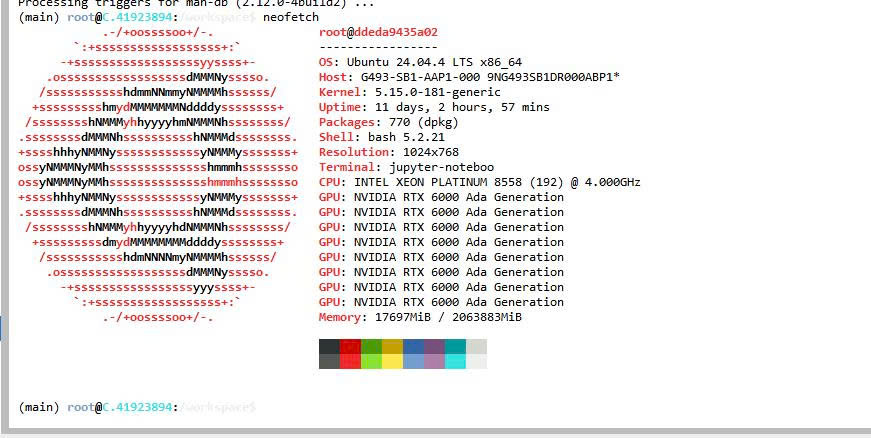
\includegraphics[width=\textwidth]{system-req.jpg}
        \caption{Chi tiết cấu hình phần cứng cấp phát}
    \end{subfigure}
    \vspace{0.5cm}
    \begin{subfigure}{0.5\textwidth}
        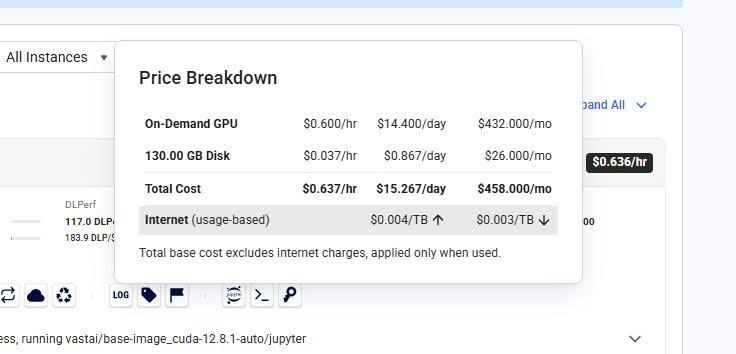
\includegraphics[width=\textwidth]{price02.jpg}
        \caption{Bảng giá \& Biên lai thuê máy chủ thực nghiệm}
    \end{subfigure}
    \caption{Tài liệu minh chứng về cấu hình và chi phí hạ tầng máy chủ}
\end{figure}

\section{Contributions}

Tiến độ dự án hiện tại là kết quả của sự phối hợp chặt chẽ và tinh thần làm việc độc lập của các thành viên trong nhóm Data \& Infrastructure. Dưới đây là các đóng góp nổi bật đã được ghi nhận qua hệ thống quản lý mã nguồn:

\subsection{Nguyễn Hồ Phát (Phat.Nguyen)}
Thành viên Nguyễn Hồ Phát chịu trách nhiệm chính trong việc thiết lập kiến trúc môi trường chạy và phát triển các bộ lọc dữ liệu cốt lõi. Cụ thể:
\begin{itemize}
    \item \textbf{Thiết lập hạ tầng Docker:} Đã hoàn thành cấu hình và setup môi trường Docker thông qua file \texttt{docker-compose.yml}, sử dụng base image \texttt{python:3.10-slim}. Việc này đảm bảo sự đồng nhất tuyệt đối về môi trường giữa máy cá nhân của các thành viên và máy chủ thực nghiệm.
    \item \textbf{Phát triển bộ lọc tiếng Việt (Vietnamese Curation Filters):} Đã nghiên cứu và lập trình các bộ lọc dữ liệu tương thích với kiến trúc NeMo Curator. Các bộ lọc này giúp xử lý các vấn đề đặc thù của tiếng Việt như ký tự Unicode rác, chuẩn hóa dấu câu, và lọc nhiễu.
    \item \textbf{Tài liệu hóa:} Khởi tạo báo cáo tiến độ Data Team chi tiết và cập nhật các xác nhận chạy thành công Docker runtime, giúp cả nhóm dễ dàng nắm bắt tiến độ.
\end{itemize}

\subsection{Huỳnh Hữu Huy (TriH28)}
Trong môi trường xử lý Big Data, chất lượng dữ liệu là yếu tố then chốt. Huỳnh Hữu Huy đã đảm nhận vai trò kiểm soát chất lượng dữ liệu:
\begin{itemize}
    \item \textbf{Xây dựng quy chuẩn (Quality Control):} Bổ sung danh sách kiểm tra chất lượng dữ liệu (Data Quality Checklist), đóng vai trò như một bộ tiêu chuẩn để đánh giá dữ liệu đầu ra.
    \item \textbf{Tối ưu quá trình kiểm thử:} Chủ động dọn dẹp (clean) bộ Vietnamese test suite và đặc biệt là phát triển thêm một tập dữ liệu nhỏ gọn (smoke dataset). Smoke dataset này cho phép nhóm thực thi kiểm thử toàn bộ luồng pipeline cực kỳ nhanh chóng mà không làm cạn kiệt tài nguyên máy tính.
\end{itemize}

\subsection{Nguyễn Đặng Quốc Anh (QUOC ANH)}
Quốc Anh là người trực tiếp khai phá các nguồn dữ liệu phức tạp trên không gian mạng và đóng gói chúng cho thực nghiệm:
\begin{itemize}
    \item \textbf{Khai phá dữ liệu đa nguồn:} Phát triển và tích hợp thành công pipeline xử lý dữ liệu cho hai nguồn quan trọng và giàu ngữ cảnh là VMLU và VTSNLP.
    \item \textbf{Tinh chỉnh dữ liệu (Calibrated Test Samples):} Dày công chuẩn bị, tinh chỉnh và đóng gói thành công 510 mẫu kiểm thử đầu ra chất lượng cao (calibrated samples). Đây sẽ là bộ tham chiếu chính xác cho bước đánh giá Perplexity và Throughput sau này.
\end{itemize}

\section{Pipeline Architecture}

Dự án hiện đang áp dụng một kiến trúc xử lý dữ liệu lai ghép (\textbf{Hybrid NeMo-compatible curation}). Kiến trúc này tận dụng điểm mạnh của cả NVIDIA NeMo Curator và tính linh hoạt của Python nhằm tối đa hóa thông lượng (throughput) xử lý văn bản:

\begin{enumerate}
    \item \textbf{Tầng NeMo Curator:} Được giao trọng trách xử lý các tác vụ có tính lặp lại cao trên khối lượng lớn tài liệu. Tầng này bao gồm các mô-đun sửa lỗi văn bản tự động (ftfy fix), chuẩn hóa Unicode về dạng chuẩn NFC, chuẩn hóa ký tự xuống dòng (newline), và áp dụng các bộ lọc heuristic.
    \item \textbf{Tầng Python Orchestration:} Đóng vai trò là "nhạc trưởng" điều phối toàn bộ luồng I/O (chủ yếu là định dạng JSONL). Python được sử dụng để thực hiện các thuật toán phức tạp đòi hỏi lưu giữ trạng thái như loại bỏ tài liệu trùng lặp tuyệt đối (\texttt{exact\_dedup}) và trùng lặp gần (\texttt{near\_dedup}). Cuối cùng, tầng này sẽ xây dựng test-set dựa trên tokenizer mục tiêu và xác thực số lượng token.
\end{enumerate}

\section{Output Analysis}

Kết quả của pipeline curation là một tập dữ liệu nhỏ gọn nhưng đa dạng về chiều dài ngữ cảnh. File kết quả \texttt{datasets/test\_set\_small.json} đã được khởi tạo thành công với đặc tả ngôn ngữ là Tiếng Việt, sử dụng Tokenizer \texttt{Qwen/Qwen2.5-7B-Instruct-1M}, và nguồn dữ liệu thô chủ yếu từ tập \texttt{VTSNLP/vietnamese\_curated\_dataset}.

Việc phân nhóm theo Context Length (4k, 8k, 16k) là vô cùng quan trọng, bởi vì lượng VRAM tiêu thụ của KV Cache sẽ tăng theo cấp số nhân (hoặc tuyến tính tùy kiến trúc) khi context length kéo dài. Bảng 2 thể hiện sự phân bổ token thống nhất cho các bài kiểm thử sắp tới.

\begin{table}[H]
\centering
\begin{tabular}{@{}ccccc@{}}
\toprule
\textbf{Nhóm Context} & \textbf{Số lượng mẫu} & \textbf{Tokens Nhỏ nhất} & \textbf{Tokens Lớn nhất} & \textbf{Trung bình} \\ \midrule
4k & 4 & 5000 & 5000 & 5000.0 \\
8k & 4 & 8099 & 9500 & 8731.5 \\
16k & 4 & 14562 & 18500 & 17255.0 \\ \bottomrule
\end{tabular}
\caption{Thống kê Test-set theo từng nhóm Context Length}
\end{table}

\section{Risk \& Suggestions}

Trong quá trình triển khai Giai đoạn 1, nhóm đã ghi nhận một số rủi ro kỹ thuật nhất định và đã lên kế hoạch xử lý trong sprint tiếp theo:

\subsection{Hạn chế \& Rủi ro}
\begin{itemize}
    \item \textbf{Gián đoạn nguồn dữ liệu:} Nguồn dữ liệu VMLU hiện đang bị từ chối truy cập (trả về lỗi HTTP 401 Unauthorized) từ máy chủ Hugging Face. Thêm vào đó, bộ dữ liệu V-Bench chưa được tích hợp do nhà cung cấp chưa cấp phát Dataset ID ổn định.
    \item \textbf{Nút thắt cổ chai (Bottleneck) hiệu suất:} Thuật toán loại bỏ trùng lặp (Deduplication) hiện vẫn đang được viết bằng thuần Python thay vì sử dụng các thư viện tăng tốc C++/CUDA của NeMo. Khi mở rộng quy mô dữ liệu lên mức hàng chục Gigabyte, quá trình này có thể gây treo hệ thống hoặc kéo dài thời gian xử lý một cách đáng kể.
\end{itemize}

\subsection{Đề xuất bước tiếp theo}
\begin{itemize}
    \item \textbf{Củng cố dữ liệu:} Nhóm sẽ nghiên cứu các bộ dữ liệu mã nguồn mở tương đương để bổ sung.
    \item \textbf{Tối ưu hóa môi trường chạy:} Đề xuất lưu trữ toàn bộ bản sao (snapshot) của tokenizer và cached model vào ổ cứng cục bộ (local). Việc này giúp các lần chạy pipeline sau không bị phụ thuộc vào tốc độ mạng.
    \item \textbf{Mở rộng độ phủ (Domain Coverage):} Tiến hành mở rộng số lượng mẫu trong test-set, bổ sung các thể loại văn bản đa dạng (y tế, pháp luật, báo chí) để kết quả benchmark có giá trị thực tiễn cao hơn.
\end{itemize}

\end{document}
